
\documentclass[12pt]{article}
 
\usepackage[margin=1in]{geometry} 
\usepackage{amsmath,amsthm,amssymb}
\usepackage{pifont}
\usepackage{graphics}
\usepackage{graphicx}
\usepackage{array}
 
\newcommand{\N}{\mathbb{N}}
\newcommand{\Z}{\mathbb{Z}}
 
\newenvironment{theorem}[2][Theorem]{\begin{trivlist}
\item[\hskip \labelsep {\bfseries #1}\hskip \labelsep {\bfseries #2.}]}{\end{trivlist}}
\newenvironment{lemma}[2][Lemma]{\begin{trivlist}
\item[\hskip \labelsep {\bfseries #1}\hskip \labelsep {\bfseries #2.}]}{\end{trivlist}}
\newenvironment{exercise}[2][Exercise]{\begin{trivlist}
\item[\hskip \labelsep {\bfseries #1}\hskip \labelsep {\bfseries #2.}]}{\end{trivlist}}
\newenvironment{problem}[2][Problem]{\begin{trivlist}
\item[\hskip \labelsep {\bfseries #1}\hskip \labelsep {\bfseries #2.}]}{\end{trivlist}}
\newenvironment{question}[2][Question]{\begin{trivlist}
\item[\hskip \labelsep {\bfseries #1}\hskip \labelsep {\bfseries #2.}]}{\end{trivlist}}
\newenvironment{corollary}[2][Corollary]{\begin{trivlist}
\item[\hskip \labelsep {\bfseries #1}\hskip \labelsep {\bfseries #2.}]}{\end{trivlist}}

\newenvironment{solution}{\begin{proof}[Solution]}{\end{proof}}
 
\begin{document}
 
% --------------------------------------------------------------
%                         Start here
% --------------------------------------------------------------
 
\title{Homework 1}
\author{Georgios Kontoudis \textbullet{} gpkont@vt.edu\\ 
AOE 5984 Cyber-Physical Systems \& Distributed Control} 
\date{Spring 2017}
 
\maketitle
\begin{exercise}{1} %theorem, exercise, problem, or question 
\textbf{Single scalar integrator dynamics for local voting protocols.}
\end{exercise}
\begin{solution}
The given graph topologies are depicted in fig \ref{graphs}. The graph topologies include a directed graph, an undirected graph, a complete graph $K^6$, a directed tree graph, an undirected star $K_{1.5}$ graph, a directed star, an undirected 6-cycle, a directed 6-cycle, and an undirected path $P^5$ respectively.
\begin{figure}[!h]
	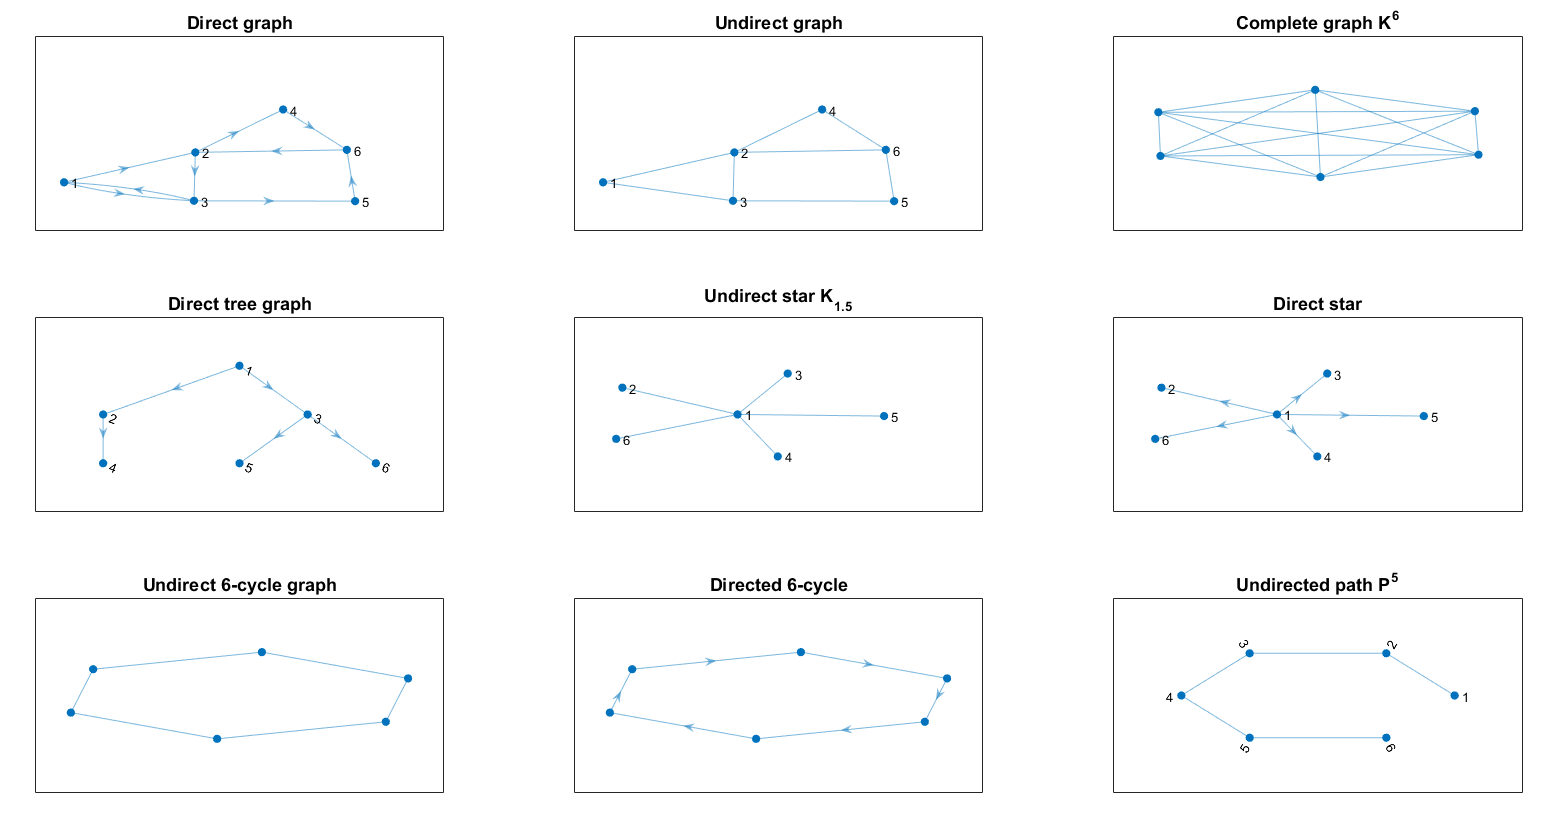
\includegraphics[scale=0.31]{figures/Graphs.png}
	\centering
	\caption{Graph topologies.}
	\label{graphs}
\end{figure}

Two different scalar single integrator dynamics of a local voting protocol with agents were simulated. First, we considered the following local voting protocol for every agent $i$
\begin{equation*}
u_i = \sum_{j \in N_i}a_{ij}(x_j-x_i)
\end{equation*}
with close-loop dynamics 
\begin{equation*}
\dot{x_i} = u_i,
\end{equation*}
which can be simplified as
\begin{equation*}
\dot{x_i} = -d_ix_i + [a_{i1}\hspace{.2cm}...\hspace{.2cm}a_{iN}]\begin{bmatrix}
x_1\\
.\\
.\\
.\\
x_N
\end{bmatrix}.
\end{equation*}

 The plots of the simulations are presented in fig. \ref{cgt1}, \ref{cgt2}. The fastest graph that converges is complete graph $K^6$, because all nodes are connected each other. Directed graph seem to converge slower than undirected, because the latter’s nodes  are considered to be connected in both directions. Moreover, when we have either directed star or directed tree graph all nodes converge to the leader, which do not change its initial state at all. 
\begin{figure}[!h]
	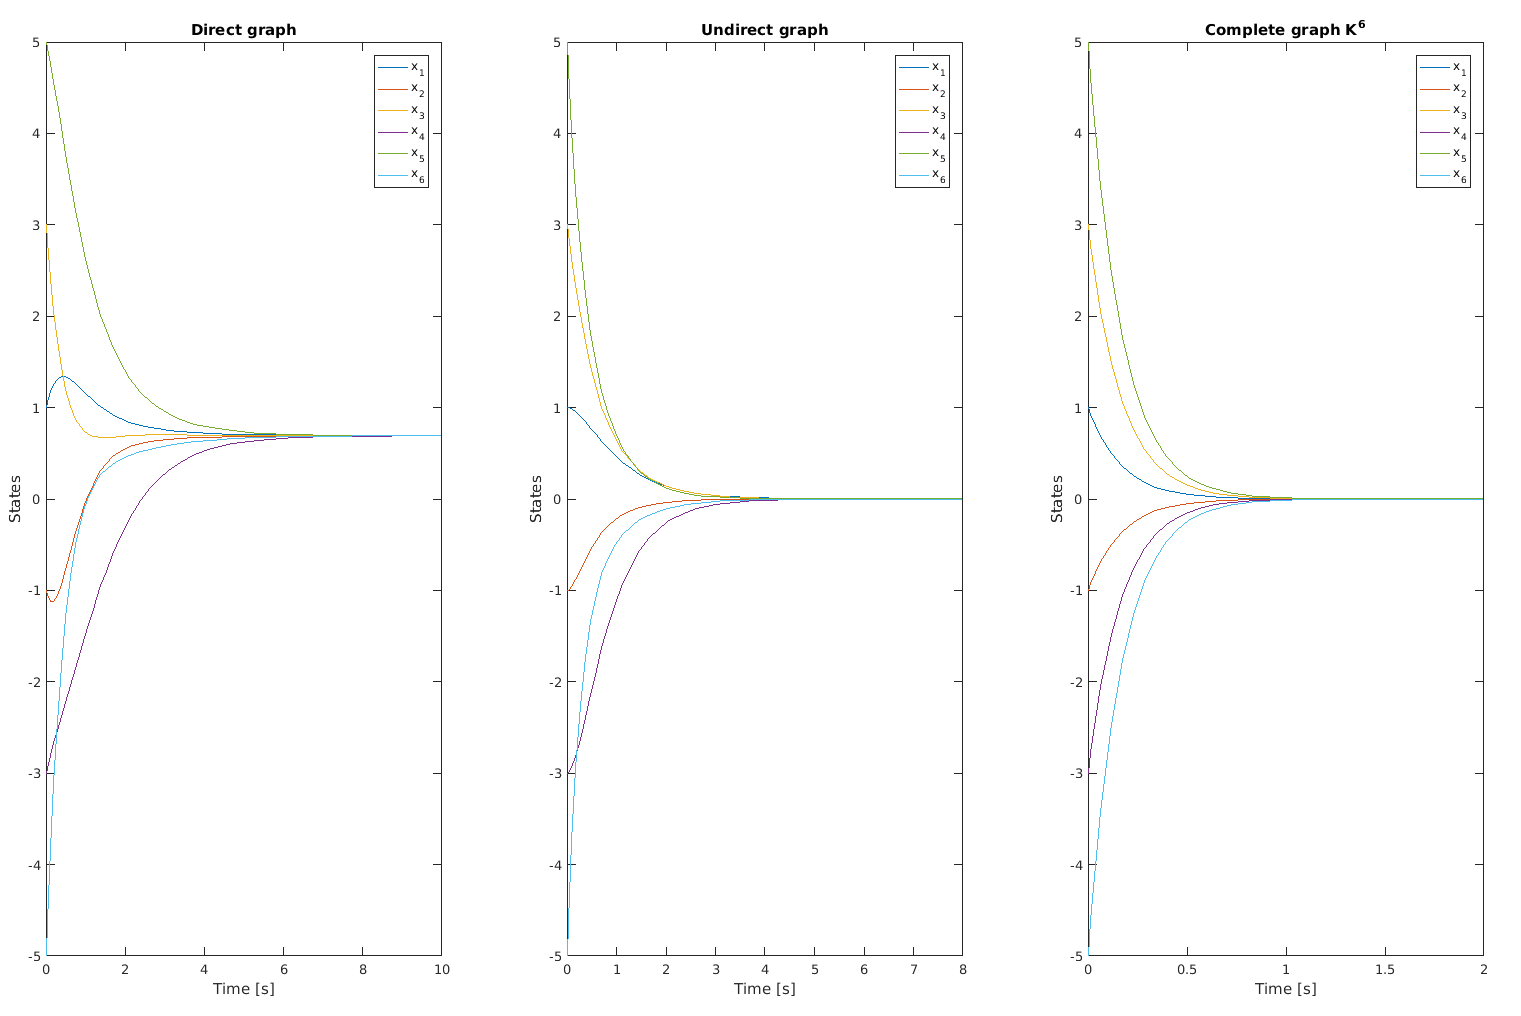
\includegraphics[scale=0.315]{figures/ConsensusGraphTopologies1.png}
	\centering
	\caption{Consensus plots for different graph topologies.}
	\label{cgt1}
\end{figure}
\begin{figure}[!t]
	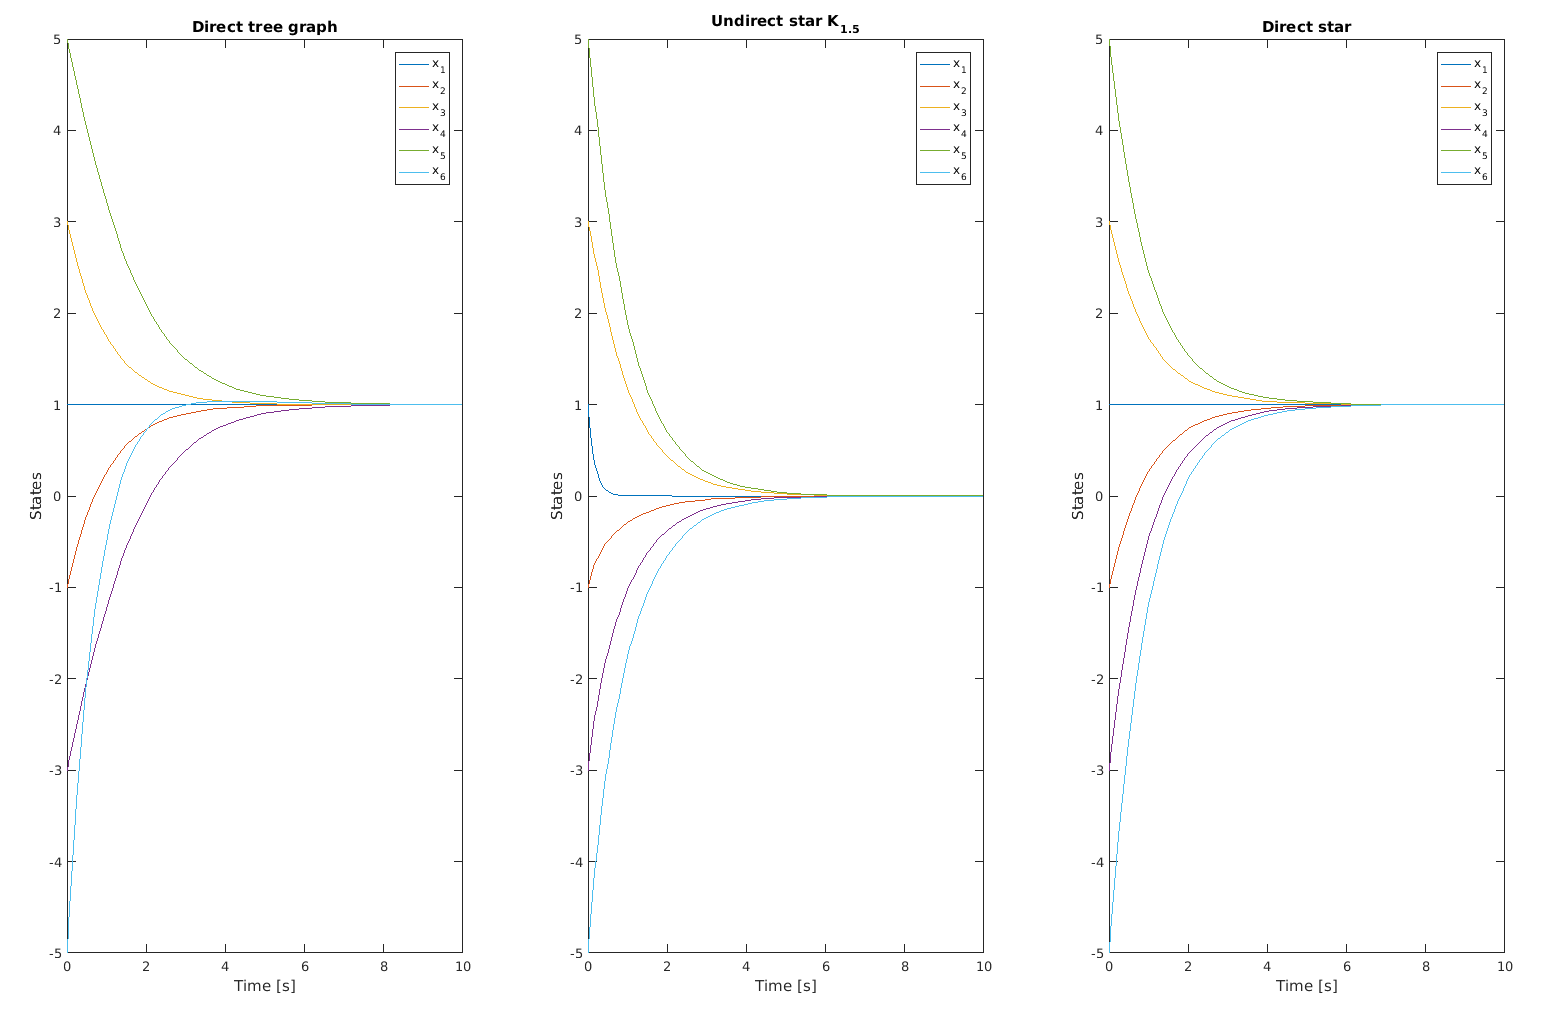
\includegraphics[scale=0.315]{figures/ConsensusGraphTopologies2.png}
	\centering
	\caption{Consensus plots for different graph topologies.}
	\label{cgt2}
\end{figure}

Then, the motion of two group agents was studied with node dynamics
\begin{equation*}
\dot{x_i}=Vcos(\theta_i),
\end{equation*}
\begin{equation*}
\dot{y_i}=Vsin(\theta_i),
\end{equation*}
\begin{equation*}
\theta_i = \sum_{j \in N_i}a_{ij}(\theta_j-theta_i).
\end{equation*}
In such case our state vector is $[x \hspace{.2cm} y \hspace{.2cm} \theta]^{\intercal}$. The plots of the simulations are presented in fig. \ref{cswarm}.
\begin{figure}[!h]
	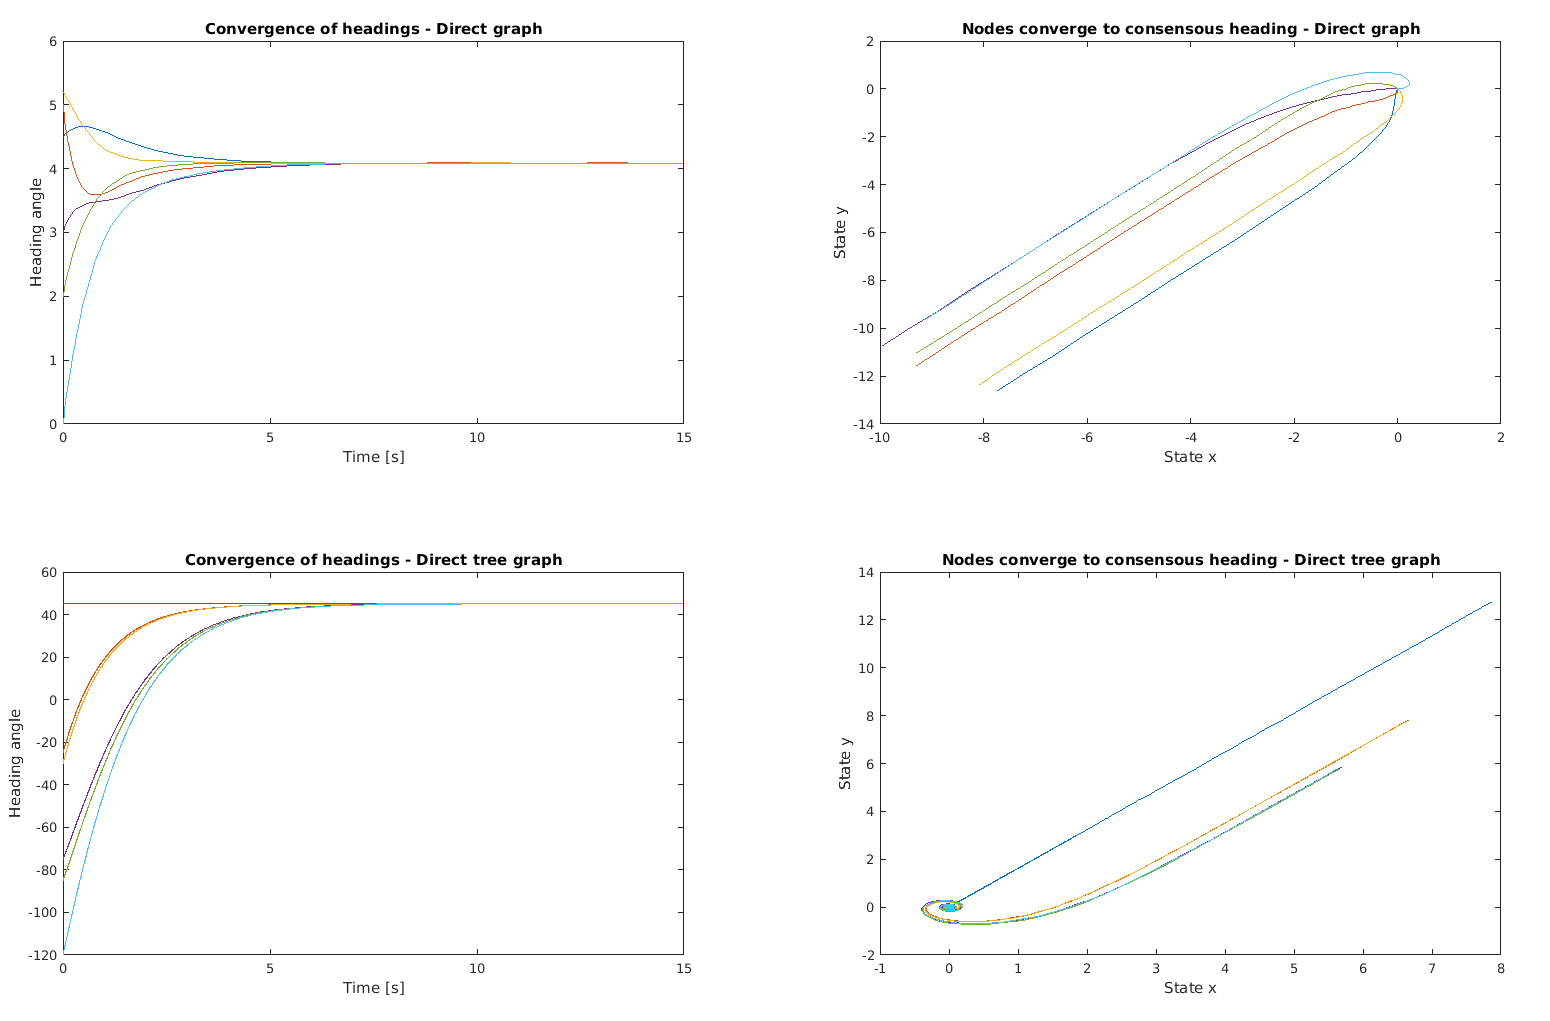
\includegraphics[scale=0.315]{figures/ConsensusSwarm.png}
	\centering
	\caption{Consensus of headings and motion consensus in (x-y) plane for direct and direct tree graph.}
	\label{cswarm}
\end{figure}

 

\end{solution}

\end{document}


